\chapter{Microkernel}

\section{Summary}
Das Micokernel Pattern wird bei Software Systemen angewendet, die sich an ändernde System Anforderungen anpassen können müssen. Es separiert einen aufs Minimum reduzierten Kern von zusätzlichen Funktionalitäten und Kunden spezifischen Teilen. Der Microkernel dient auch als Socket für diese Erweiterungen und er koordiniert ihre Zusammenarbeit.
\section{Context}
Entwicklung von mehreren Applikationen welche ähnliche Interfaces verwenden, welche auf der selben Grundfunktionalität aufbauen.
\section{Problem}
Software für ein Anwendungsgebiet zu entwickeln, welches mit einem breiten Spektrum von ähnlichen Standards und Technologien umgehen muss ist nicht einfach. Oft wird noch eine lange Lebenszeit gefordert, in welcher neue Technologien aufkommen und alte sich verändern. Das typische Beispiel für solche Software sind Betriebssysteme. Folgende Forces benötigen spezielle Aufmerksamkeit beim Design solcher Software:
\begin{itemize}
	\item Kontinuierliche Hardware und Software Evolution
	\item Einfache Portabilität, Erweiterbarkeit und einfache Integration von neuen Technologien
\end{itemize}

\section{Solution}
Das Microkernel Pattern schafft Abhilfe für oben erwähnte Probleme. Dabei werden die fundamentalen Services einer Applikationsplattform in eine Microkernel Komponente gepackt. Der Microkernel bietet anderen Komponenten die in separaten Prozessen laufen, die Möglichkeit miteinander zu kommunizieren. Er verwaltet ausserdem System weite Ressourcen, und er bietet Interfaces die anderen Komponenten Zugriff auf seine Funktionen bieten.
\subsection{Structure}
Das Microkernel Pattern definiert fünf Arten von teilnehmenden Komponenten, welche im folgenden kurz erklärt werden.
\paragraph{Microkernel} Der Microkernel repräsentiert die Hauptkomponente des Patterns. Er implementiert zentrale Services für die Kommunikation und Handhabung von Ressourcen. Alle anderen Komponenten bauen auf den Interfaces die der Microkernel für diese Services bietet, auf. Viele System spezifische Abhängigkeiten (Bsp. Hardware) sind im Microkernel vor den anderen Komponenten versteckt.
\paragraph{Internal Server} Internal Servers sind separate Komponenten welche die Funktionalität des Mikrokernels erweitern. Der Microkernel ruft die Funktionalität des Servers via Service Request auf. Internal Servers können also auch gewisse Abhängigkeiten zum darunterliegenden Software System haben. Ein Beispiel für ein Internal Server wären Grafikkarten Treiber für spezifische Modelle. Internal Servers können als Erweiterungen des Microkernels, welche nur bei Bedarf geladen werden und nur vom Microkernel zugreifbar sind, gesehen werden.
\paragraph{External Server} Als External Server wird eine Komponente bezeichnet, welche auf die Interfaces des Microkernels zugreift und darauf eine eigene View aufbaut. Externe Server laufen in separaten Prozessen und bieten selbst wiederum Interfaces an. Sie erhalten Service Requests über den Kommunikations Service des Microkernels.
\paragraph{Client} Ein Client ist eine Applikation die mit genau einem External Server in Bezug steht. Clients implementieren oft das Adapter Pattern um flexibler auf Änderungen am External Server reagieren zu können. \\
Das folgende Diagramm zeigt die statische Struktur eines Microkernel Systems mit den zuvor erläuterten Komponenten:
\begin{figure}[H]
	\centering
	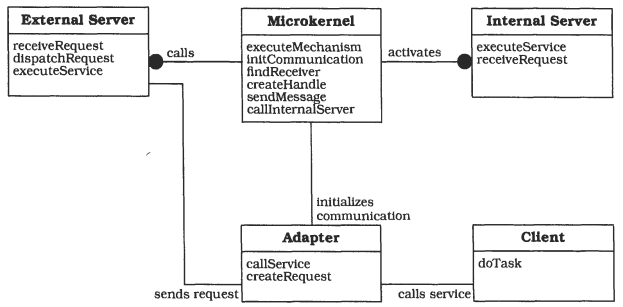
\includegraphics[width=0.7\textwidth]{figures/05-microkernel-1}
	\caption{Microkernel Struktur}
\end{figure}
\section{Consequences}
\begin{itemize}
    \pro{Portability}
    \pro{Flexibility and Extensibility}
    \pro{Separation of Policy and Mechanism}
    \pro{Scaleability}
    \pro{Reliability}
    \pro{Transparancy}
    \con{Performance}
    \con{Complexity of Design and Implementation}
\end{itemize}

\section{Known Uses}
\begin{itemize}
	\item Windows NT
	\item Chorus OS
	\item MKDE (Microkernel Database Engine)
\end{itemize}

\section{Relationships}
\begin{itemize}
	\item \textit{Broker Pattern}
	\item \textit{Reflection Pattern} 
	\item \textit{Layers Pattern}
\end{itemize}

\section{Exam Questions}
\begin{itemize}
  \item Behauptung: dies ist eine Behauptung? (Lösung)
    \item Frage: Dies ist eine Frage? (Lösung)
\end{itemize}
